% ============================================================
% Chapter 19 --- Jordan measure and the Riemann integral
% Originally: content/week-08.tex, \section{Multivariate integration} (Corsin Week 8),
%             with problems 8.2 and 8.4 from sheet 8.
% ============================================================
\chapter{Jordan Measure and the Riemann Integral}
\label{ch:jordan_measure}

% Transition: Claude Opus 5 (Medium)
Integration in several variables needs a notion of the volume of a domain before it can define an
integral over one. This chapter sets up Jordan measure and the multidimensional Riemann integral
built on it, and then spends most of its effort on the sets that are \emph{not} Jordan
measurable. That is where every counterexample on the problem sheet lives, and the reason they
exist is a single one: a Jordan cover may use only finitely many cubes, all of one size. A short
section extends the integral to unbounded domains, which every later chapter uses and none of them
defines. The chapter closes with a digression on the Lebesgue theory, which repairs that single
defect properly; it is stated without proofs and used nowhere afterwards.

% Originally: content/week-08.tex, \section{Multivariate integration} (Corsin Week 8)

% Source: Corsin Nick/Class Notes/Week 8.pdf, p. 7
\section{Multivariate integration}
\label{sec:multivariate_integration}

% Supplement: Sascha Brack/Class Notes/Week_08_Notes_Monday.pdf, pp. 5--7
\subsection{Jordan measure and the Riemann integral}
The rigorous definition of the multidimensional integral relies on the \newterm{Jordan measure} (\germanterm{Jordan-Maß}). The intuition, as presented in Sascha Brack's notes, involves \qt{dyadic cubes} (pixels) that approximate a region from the inside and outside.

\begin{center}
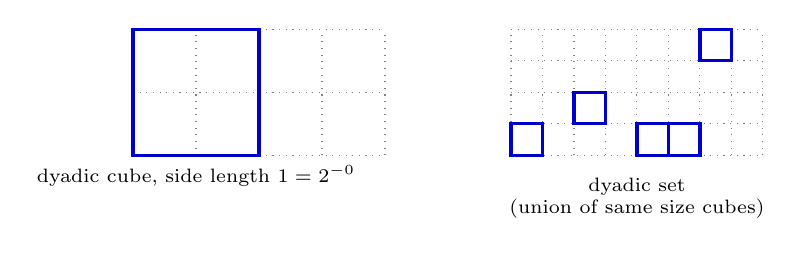
\begin{tikzpicture}[scale=0.8]
  % first grid
  \draw[gray, dotted] (0,0) grid (4,2);
  \draw[very thick, blue!80!black] (0,0) rectangle (2,2);
  \node[below, font=\scriptsize] at (1,0) {dyadic cube, side length $1=2^{-0}$};
  
  \begin{scope}[shift={(6,0)}]
    \draw[gray, dotted, step=0.5] (0,0) grid (4,2);
    \draw[very thick, blue!80!black] (0,0) rectangle (0.5,0.5);
    \draw[very thick, blue!80!black] (1,0.5) rectangle (1.5,1.0);
    \draw[very thick, blue!80!black] (2,0) rectangle (2.5,0.5);
    \draw[very thick, blue!80!black] (2.5,0) rectangle (3.0,0.5);
    \draw[very thick, blue!80!black] (3,1.5) rectangle (3.5,2.0);
    \node[below, font=\scriptsize, align=center] at (2,-0.2) {dyadic set\\(union of same size cubes)};
  \end{scope}
\end{tikzpicture}
\end{center}

% Generator: Claude Opus 5 (High) --- the notion was used throughout this chapter and in
% \cref{ch:change_of_variables} but had no numbered definition to point at.
\begin{definition}[Dyadic cube and dyadic set]
\label{def:dyadic_set}
For $p \in \mathbb{N}$ and $a \in \mathbb{Z}^n$, the \newterm{dyadic cube}
(\germanterm{dyadischer Würfel}) of generation $p$ at $a$ is
\[Q_p(a) := 2^{-p}\big(a + [0,1)^n\big),\]
a half-open cube of side length $2^{-p}$. A \newterm{dyadic set} (\germanterm{dyadische Menge})
is a finite union $E = \bigcup_{\ell=1}^N Q_p(a(\ell))$ of distinct dyadic cubes \emph{of one
common generation} $p$, and its volume is
\[\mu(E) := 2^{-pn}N.\]
\end{definition}

The requirement that all cubes share a generation is not cosmetic: it is what separates the
Jordan theory from the Lebesgue theory, as \cref{rem:jordan_vs_lebesgue_sizes} makes precise.

% Supplement: Sascha Brack/Class Notes/Week_08_Notes_Monday.pdf, pp. 5--7
Similar to the 1D Riemann integral, we approximate the volume of a set $E \subseteq \mathbb{R}^n$ using an outer sequence of dyadic sets $G_i \supseteq E$ and an inner sequence $F_i \subseteq E$. If the limits of their volumes coincide as the pixel size $2^{-p} \to 0$, $E$ is \newterm{Jordan measurable}.

Furthermore, the multidimensional integral of a non-negative function $f : A \to \mathbb{R}$ is exactly the $(n+1)$-dimensional Jordan measure (volume) of its hypograph $\Gamma_A(f)$:

\begin{center}
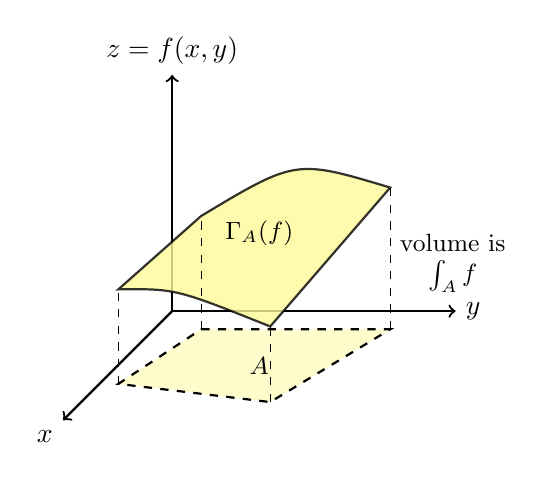
\begin{tikzpicture}[scale=1.2]
  % axes
  \draw[->, thick] (0,0,0) -- (3,0,0) node[right] {$y$};
  \draw[->, thick] (0,0,0) -- (0,2.5,0) node[above] {$z = f(x,y)$};
  \draw[->, thick] (0,0,0) -- (0,0,3) node[below left] {$x$};
  
  % base domain A
  \draw[thick, dashed, fill=yellow!20] (0.5,0,0.5) -- (2.5,0,0.5) -- (2.0,0,2.5) -- (0.2,0,2.0) -- cycle;
  \node[font=\small] at (1.5, 0, 1.5) {$A$};
  
  % top surface graph(f)
  \draw[thick, fill=yellow!40, opacity=0.8] (0.5,1.2,0.5) .. controls (1.5,1.8,0.5) .. (2.5,1.5,0.5)
    -- (2.0,0.8,2.5) .. controls (1.0,1.2,2.5) .. (0.2,1.0,2.0) -- cycle;
  \node[font=\small] at (1.5, 1.4, 1.5) {$\Gamma_A(f)$};
  
  % vertical lines
  \draw[dashed] (0.5,0,0.5) -- (0.5,1.2,0.5);
  \draw[dashed] (2.5,0,0.5) -- (2.5,1.5,0.5);
  \draw[dashed] (2.0,0,2.5) -- (2.0,0.8,2.5);
  \draw[dashed] (0.2,0,2.0) -- (0.2,1.0,2.0);
  
  \node[right, font=\small, align=center] at (2.5, 0.7, 0.5) {volume is\\$\int_A f$};
\end{tikzpicture}
\end{center}

% Source: Jérôme Paschoud/Notizen/Woche 8.2 Riemann-Integral.pdf, p. 1
% Generator: Gemini 3.1 Pro (High)
\begin{definition}[Riemann integral in $\mathbb{R}^n$]
\label{def:riemann_integral_rn}
Let $A \subseteq \mathbb{R}^n$ and $f: A \to \mathbb{R}$. Analogous to Analysis I, the integral is defined via dyadic step functions (\germanterm{dyadische Treppenfunktionen}). The lower and upper integrals are defined as
\begin{align*}
  \underline{\int}_A f &:= \sup \left\{ \int_A g \;\middle|\; g: \mathbb{R}^n \to \mathbb{R} \text{ dyadic step function with } g \leq f \right\}, \\
  \overline{\int}_A f &:= \inf \left\{ \int_A h \;\middle|\; h: \mathbb{R}^n \to \mathbb{R} \text{ dyadic step function with } h \geq f \right\}.
\end{align*}
The function $f$ is \newterm{Riemann integrable} if $\underline{\int}_A f = \overline{\int}_A f$. In this case, their common value is denoted by $\int_A f$.

\begin{center}
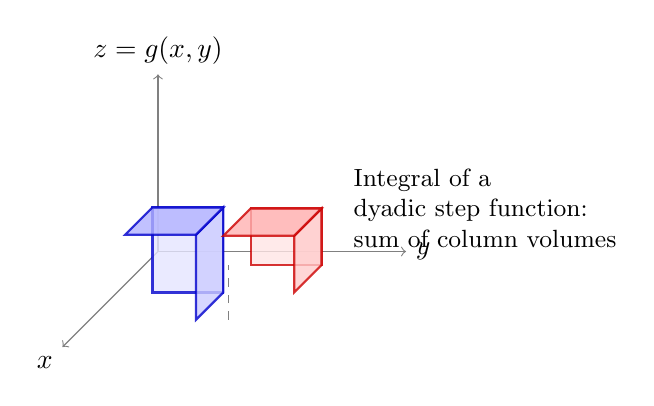
\begin{tikzpicture}[scale=0.9]
  % axes
  \draw[->, gray] (0,0,0) -- (3.5,0,0) node[right, text=black] {$y$};
  \draw[->, gray] (0,0,0) -- (0,2.5,0) node[above, text=black] {$z = g(x,y)$};
  \draw[->, gray] (0,0,0) -- (0,0,3.5) node[below left, text=black] {$x$};
  
  % Base squares
  \draw[gray, dashed] (0.5,0,0.5) grid (2.5,0,2.5);
  
  % Column 1
  \draw[thick, blue!80!black, fill=blue!10, opacity=0.8] (0.5,0,1.5) -- (0.5,1.2,1.5) -- (1.5,1.2,1.5) -- (1.5,0,1.5) -- cycle;
  \draw[thick, blue!80!black, fill=blue!20, opacity=0.8] (1.5,0,1.5) -- (1.5,1.2,1.5) -- (1.5,1.2,2.5) -- (1.5,0,2.5) -- cycle;
  \draw[thick, blue!80!black, fill=blue!30, opacity=0.8] (0.5,1.2,1.5) -- (1.5,1.2,1.5) -- (1.5,1.2,2.5) -- (0.5,1.2,2.5) -- cycle;
  
  % Column 2
  \draw[thick, red!80!black, fill=red!10, opacity=0.8] (1.5,0,0.5) -- (1.5,0.8,0.5) -- (2.5,0.8,0.5) -- (2.5,0,0.5) -- cycle;
  \draw[thick, red!80!black, fill=red!20, opacity=0.8] (2.5,0,0.5) -- (2.5,0.8,0.5) -- (2.5,0.8,1.5) -- (2.5,0,1.5) -- cycle;
  \draw[thick, red!80!black, fill=red!30, opacity=0.8] (1.5,0.8,0.5) -- (2.5,0.8,0.5) -- (2.5,0.8,1.5) -- (1.5,0.8,1.5) -- cycle;

  \node[font=\small, align=left] at (5, 1, 1) {Integral of a\\dyadic step function:\\sum of column volumes};
\end{tikzpicture}
\end{center}

This integral satisfies all the \qt{good} properties from the one-dimensional case, such as linearity. Moreover, if $E \subseteq \mathbb{R}^n$ is Jordan measurable and $f: \overline{E} \to [0, \infty)$ is continuous, then $f$ is Riemann integrable on $E$.
\end{definition}

% Source: Diego Torres Tejeda/Notes - 17.04 - Diego Torres Tejeda.pdf, p. 1
% Generator: Gemini 3.6 Flash (High)
\begin{theorem}[Jordan measurability criterion via boundary]
\label{thm:jordan_measurability_boundary_criterion}
A bounded subset $E \subseteq \mathbb{R}^n$ is Jordan measurable if and only if its boundary $\partial E$ is a Jordan null set, i.e.\ $\mu_{\mathrm{out}}(\partial E) = 0$.
\end{theorem}

\begin{lemma}[Compact sets: Jordan null versus Lebesgue null]
\label{lem:compact_jordan_vs_lebesgue_null}
Let $K \subseteq \mathbb{R}^n$ be compact. Then $K$ is a Jordan null set if and only if $K$ is a Lebesgue null set.
\end{lemma}

\begin{proof}
If $K$ is Jordan null, then for every $\varepsilon > 0$, $K$ is covered by finitely many dyadic cubes $Q_1, \dots, Q_m$ with total volume $\sum_{i=1}^m \mu(Q_i) < \varepsilon$, so $K$ is a Lebesgue null set. Conversely, if $K$ is Lebesgue null, there is a countable cover by dyadic cubes $\{Q_j\}_{j \ge 1}$ with $\sum_{j=1}^\infty \mu(Q_j) < \varepsilon$. Taking the interiors of slightly enlarged cubes yields an open cover of the compact set $K$, which admits a finite subcover of total volume $< 2\varepsilon$, proving $K$ is Jordan null.
\end{proof}

% Source: Diego Torres Tejeda/Notes - 17.04 - Diego Torres Tejeda.pdf, pp. 3--4
% Generator: Gemini 3.6 Flash (High)
\begin{example}[The Cantor set is a Jordan null set]
\label{ex:cantor_set_jordan_null}
Consider the middle-thirds \newterm{Cantor set} $C \subseteq [0,1]$, defined inductively by $C_0 := [0,1]$ and
\[
C_{n+1} := \tfrac{1}{3} C_n \cup \left( \tfrac{2}{3} + \tfrac{1}{3} C_n \right), \qquad C := \bigcap_{n=0}^\infty C_n.
\]
Each $C_n$ consists of $2^n$ closed intervals of length $3^{-n}$, so $\mu(C_n) = (2/3)^n$. Since $C \subseteq C_n$ for all $n$, we have
\[
\mu_{\mathrm{out}}(C) \leq \mu(C_n) = \left(\tfrac{2}{3}\right)^n \xrightarrow{n\to\infty} 0,
\]
proving that the Cantor set $C$ is a Jordan null set.

Moreover, as Diego Torres Tejeda highlights in his notes, $C$ consists precisely of those points $x \in [0,1]$ possessing a ternary (base-3) expansion $x = \sum_{n=1}^\infty \frac{a_n}{3^n}$ composed entirely of digits $a_n \in \{0, 2\}$ without the digit $1$.
\end{example}

% Source: Diego Torres Tejeda/Notes - 17.04 - Diego Torres Tejeda.pdf, p. 5
% Generator: Gemini 3.6 Flash (High)
\begin{example}[An open set that is not Jordan measurable]
\label{ex:non_jordan_measurable_open_set}
Jordan measurability can fail even for open sets. Enumerate the rational numbers in $[0,1]$ as $\mathbb{Q} \cap [0,1] = \{q_1, q_2, \dots\}$, and define the open set
\[
U := \bigcup_{k=1}^\infty B_{2^{-(k+2)}}(q_k) \;\cap\; (0,1).
\]
Since $\mathbb{Q} \cap [0,1]$ is dense in $[0,1]$, the closure of $U$ is $\overline{U} = [0,1]$. If $U$ were Jordan measurable, its measure would satisfy $\mu(U) = \mu(\overline{U}) = 1$. However, any finite union of intervals covering a dyadic inner approximation of $U$ has measure bounded by $\sum_{k=1}^\infty 2 \cdot 2^{-(k+2)} = \frac{1}{2}$. Thus $\mu_{\mathrm{in}}(U) \leq \frac{1}{2} < 1 = \mu_{\mathrm{out}}(U)$, showing that $U$ is \textbf{not} Jordan measurable. Its boundary $\partial U = [0,1] \setminus U$ is a \qt{fat} boundary of positive outer measure.
\end{example}

% Source: Jérôme Paschoud/Notizen/Woche 8.1 Tangentialräume und Jordan Mass.pdf, p. 3
% Generator: Gemini 3.1 Pro (High)
\begin{proposition}[Algebra of Jordan measurable sets]
\label{prop:algebra_jordan_measurable}
If $E, F \subset \mathbb{R}^n$ are Jordan measurable, then their union $E \cup F$, intersection $E \cap F$, and differences $E \setminus F$, $F \setminus E$ are also Jordan measurable.
Furthermore, if $E \cap F = \emptyset$ (or if they only intersect in a Jordan null set), then
\[
\mu(E \cup F) = \mu(E) + \mu(F).
\]
\end{proposition}

% Source: Jérôme Paschoud/Notizen/Woche 8.1 Tangentialräume und Jordan Mass.pdf, p. 4
% Generator: Gemini 3.1 Pro (High)
\begin{remark}[Lebesgue null vs.\ Jordan null]
\label{rem:lebesgue_vs_jordan_null}
A set $E \subset \mathbb{R}^n$ is \newterm{Lebesgue null} if for every $\varepsilon > 0$, there exist \emph{countably} many dyadic cubes $Q_i$ covering $E$ with $\sum \mu(Q_i) < \varepsilon$. For a \newterm{Jordan null} set, the cover must be formed by \emph{finitely} many cubes (which implicitly requires $E$ to be bounded).
Because a countable cover is allowed, the set $\mathbb{Q} \cap [0,1]$ is Lebesgue null. However, it is not Jordan null (in fact, it is not even Jordan measurable, as seen in \cref{ex:non_jordan_measurable_open_set}), since any finite union of intervals covering it must also cover its closure $[0,1]$, thus having measure at least $1$.
\end{remark}

% Quelle: Linus Lüchinger/Slides/Slides-04-16.pdf, slide 6
% Generator: Claude Opus 5 (High)
\begin{remark}[The relaxation is really about \emph{sizes}, not just counts]
\label{rem:jordan_vs_lebesgue_sizes}
Stating the difference as \qt{finitely many} against \qt{countably many} is correct but hides
where the extra power actually comes from. A Jordan cover is a \emph{dyadic set}, and every cube
in a dyadic set of generation $p$ has the same side length $2^{-p}$
(\cref{def:dyadic_set}). So the two conditions really read:
\begin{itemize}
  \item \textbf{Jordan null:} for each $\varepsilon>0$, cover $E$ by cubes that all have
    \emph{one common side length}, of total volume $<\varepsilon$. Finiteness is then automatic:
    only finitely many cubes of a fixed size fit into a bounded region.
  \item \textbf{Lebesgue null:} for each $\varepsilon>0$, cover $E$ by cubes of \emph{whatever
    side lengths you like}, of total volume $<\varepsilon$. Allowing the sizes to vary is exactly
    what lets the cover be infinite while the total volume stays finite.
\end{itemize}
The two relaxations are therefore one relaxation. It is permission to shrink the cubes as you go
that buys the countable cover, and it is the countable cover that makes the notions differ.

$\mathbb{N} \subseteq \mathbb{R}$ shows this in its purest form. Cover the integer $k$ by an
interval of length $\varepsilon\,2^{-k-1}$; the total length is $\varepsilon$, so $\mathbb{N}$ is
Lebesgue null. No Jordan cover can do this: cubes of one fixed length $2^{-p}$ need at least one
cube per integer, infinitely many of them, of infinite total length. (Indeed $\mathbb{N}$ is
unbounded, so it is not Jordan measurable at all.) The point is that the geometric series is
available only when the sizes may vary.
\end{remark}

% Source: Jérôme Paschoud/Notizen/Woche 8.1 Tangentialräume und Jordan Mass.pdf, p. 4
% Generator: Gemini 3.1 Pro (High)
\begin{theorem}[Linear transformations of Jordan measurable sets]
\label{thm:jordan_measure_linear_transformation}
Let $L: \mathbb{R}^n \to \mathbb{R}^n$ be a linear, invertible map. If $E \subset \mathbb{R}^n$ is Jordan measurable, then the image $L(E)$ is also Jordan measurable, and its measure scales by the absolute value of the determinant of $L$:
\[
\mu(L(E)) = |\det L| \, \mu(E).
\]
\end{theorem}


% --- exercises relocated here from the dissolved sheet 8 ---

% Originally: content/week-08.tex, \exercisesheet{8}, problem 8.2
% Source: exercises/Ex8_Analysis2_eng.pdf

% Source: exercises/Ex8_Analysis2_eng.pdf, p. 1
\begin{exercise}[8.2 --- True or False \textnormal{(important)}]
\label{ex:8.2}
\begin{enumerate}[label=\textbf{\arabic*.}]
  \item A bounded countable set is always Jordan-null.
  \item A countable set is always Lebesgue-null.
  \item Let $D \subset [0,1]$ be a dense set (i.e.\ $\overline D = [0,1]$). Then
    $\mu_{out}(D) = 1$. ($\mu_{out}$ was defined in Definition 13.10.)
  \item Let $X, Y \subset [0,1]$ Jordan measurable sets such that $\mu(X) > 1/2$ and
    $\mu(Y) > 1/2$. Then $X \cap Y \neq \emptyset$.
  \item Let $X, Y \subset [0,1]$ such that $\mu_{out}(X) > 1/2$ and $\mu_{out}(Y) > 1/2$. Then
    $X \cap Y \neq \emptyset$.
\end{enumerate}
\textit{Official hint:} \textbf{8.2.5} --- $\mu_{out}$ can be positive and large on very sparse
sets\dots

% Supplement: Sascha Brack/Ex Sheet Hints/Ex8_Analysis2_hints.pdf, p. 1
\textit{Sascha Brack's hints:} a toolkit of sets worth testing every part against ---
$\mathbb{Q}$, the irrationals $\mathbb{R}\setminus\mathbb{Q}$, $\mathbb{Q}\cap[0,1]$, and
$(\mathbb{R}\setminus\mathbb{Q})\cap[0,1]$. For \textbf{8.2.3} specifically: monotonicity already
gives $\mu_{out}(D) \leq \mu_{out}([0,1]) = 1$, so the work is showing
$\mu_{out}(D) \geq 1$ --- essentially, that the \qt{smallest} dyadic set containing $D$ also
contains $[0,1]$.
\end{exercise}

% Originally: content/week-08.tex, \exercisesheet{8}, problem 8.4
% Source: exercises/Ex8_Analysis2_eng.pdf

% Source: exercises/Ex8_Analysis2_eng.pdf, p. 1
\begin{exercise}[8.4 --- Multiple Choice \textnormal{(important)}]
\label{ex:8.4}
Let $U \subset \mathbb{R}^n$ be a nonempty, open subset, $f : U \to \mathbb{R}^m$ a function,
and $N \subset U$ a Jordan null set. In which of the following cases is the image
$f(N) \subset \mathbb{R}^m$ necessarily a null set? \textit{Attention: Only one answer is
correct!}
\begin{enumerate}[label=\textbf{\arabic*.}]
  \item If $f$ is uniformly continuous.
  \item If $f$ is uniformly continuous and $m \geq n$.
  \item If $f$ is locally Lipschitz continuous.
  \item If $f$ is locally Lipschitz continuous and $m \geq n$.
\end{enumerate}
\end{exercise}

% Originally: new section (no predecessor in the week-based skeleton, and none in any tutor's
% notes). Added 2026-08-10 after a pass over lec_notes.pdf found that this document uses improper
% multidimensional integrals in at least four places without ever defining one:
%   * ex:improper_integral_polar (ch. 20) states outright that "its Riemann improper integral is
%     well-defined", which is a claim about a definition we did not have;
%   * ex:gaussian_integral_polar (ch. 20) integrates over all of R^2;
%   * ex:ai_frullani (ch. 20) integrates over the half-line;
%   * ex:10.3 (ch. 21), Gabriel's horn, integrates over [1, infinity).
% The lecture notes devote two pages to it and no tutor covers it, so this is a genuine gap
% rather than a deliberate skip. Corsin never reaches it either.

% Supplement: lec_notes.pdf, pp. 124--125
\section{Improper integrals}
\label{sec:improper_integrals}

Everything so far has integrated a continuous function over a \emph{bounded} Jordan measurable
set. Two situations fall outside that and both occur constantly in practice: the domain may be
unbounded, and the integrand may be unbounded near the edge of its domain. What should
$\int_{\mathbb{R}^2}f$ mean?

The answer avoids limits entirely, at the cost of one hypothesis.

\begin{definition}[Improper integral]
\label{def:improper_integral}
Let $U \subseteq \mathbb{R}^n$ be open and let $f \in C^0(U)$ be \textbf{non-negative}. The
\newterm{improper integral} \germanfor{uneigentliches Integral} of $f$ over $U$, still written
$\int_U f$, is
\[\int_U f := \sup\left\{\int_K f \ \middle|\ K \subseteq U \text{ compact and Jordan
  measurable}\right\} \ \in\ [0,+\infty].\]
\end{definition}

Each $\int_K f$ on the right is an ordinary integral: $K$ is compact and Jordan measurable and
$f$ is continuous on it, so \cref{def:riemann_integral_rn} applies. The supremum of a set of
real numbers bounded below by $0$ always exists in $[0,+\infty]$, so $\int_U f$ is always
defined. It may be $+\infty$, and in that case one says the improper integral \newterm{diverges}.

\begin{remark}[Why non-negativity, and what it buys]
\label{rem:improper_needs_nonnegativity}
The hypothesis $f \geq 0$ is not a technicality that a more careful definition would remove. It
is what makes the supremum monotone, so that enlarging $K$ can only increase $\int_K f$, and
that monotonicity is the whole of \cref{lem:improper_integral_as_limit} below.

Drop it and the value stops being well defined. For a sign-changing $f$ one can arrange
exhaustions that pick up the positive part faster or slower than the negative part and obtain
different answers, exactly as a conditionally convergent series can be rearranged to any sum.
\Cref{ex:feynman_dirichlet_integral} is the case in point: $\int_0^\infty (\sin x)/x\,dx = \pi/2$
is \emph{not} an improper integral in the sense above, since $(\sin x)/x$ changes sign infinitely
often and $\int_0^\infty \lvert\sin x\rvert/x\,dx = +\infty$. Its value depends on integrating in
the order $\int_0^R$ and then letting $R \to \infty$, which is why that example needs a
justification the others do not.
\end{remark}

The definition is clean but useless for computing, since one cannot take a supremum over all
compact subsets by hand. The next result says that any single sensible exhaustion suffices, and
that it does not matter which one is chosen.

\begin{lemma}[Improper integrals as limits]
\label{lem:improper_integral_as_limit}
Let $U \subseteq \mathbb{R}^n$ be open and $f \in C^0(U)$ non-negative. Let
$K_1 \subseteq K_2 \subseteq K_3 \subseteq \cdots$ be compact Jordan measurable sets with
\[\bigcup_{\ell=1}^\infty \operatorname{int}(K_\ell) = U.\]
Then
\[\int_U f = \lim_{\ell\to\infty}\int_{K_\ell} f,\]
and in particular the limit exists in $[0,+\infty]$.
\end{lemma}

\begin{proof}
Since the $K_\ell$ are nested and $f \geq 0$, the sequence $\int_{K_\ell}f$ is non-decreasing, so
it converges in $[0,+\infty]$; call the limit $\Lambda$.

\textbf{$\int_U f \leq \Lambda$.} Let $K \subseteq U$ be compact and Jordan measurable. The sets
$\operatorname{int}(K_\ell)$ are open and cover $U$, hence cover $K$, so by compactness finitely
many of them suffice; since they are nested, a single one does, say
$K \subseteq \operatorname{int}(K_{\ell_0}) \subseteq K_{\ell_0}$. Non-negativity then gives
$\int_K f \leq \int_{K_{\ell_0}} f \leq \Lambda$. Taking the supremum over all such $K$ yields
$\int_U f \leq \Lambda$.

\textbf{$\Lambda \leq \int_U f$.} Each $K_\ell$ is itself compact and Jordan measurable and
contained in $U$, so it competes in the supremum defining $\int_U f$. Consequently
$\int_{K_\ell} f \leq \int_U f$ for every $\ell$, and letting $\ell \to \infty$ gives
$\Lambda \leq \int_U f$.
\end{proof}

\begin{remark}[What the lemma licenses]
\label{rem:improper_exhaustion_free_choice}
Read the two halves together: the value does not depend on the exhaustion, so one may choose
whichever exhaustion makes the computation easy. That is the licence
\cref{ex:improper_integral_polar} and \cref{ex:gaussian_integral_polar} were already using when
they integrated over $\mathbb{R}^2$ in polar coordinates, and it is what
\cref{ex:ai_gaussian_two_exhaustions} makes explicit by running two different exhaustions against
each other and comparing the answers.
\end{remark}

\begin{aiexercise}[The Gaussian integral, two exhaustions at once]
% Generator: Claude Opus 5 (High)
\label{ex:ai_gaussian_two_exhaustions}
Let $f(x,y) := e^{-(x^2+y^2)}$ on $U := \mathbb{R}^2$, which is continuous and positive, and put
$I := \int_{-\infty}^{\infty} e^{-t^2}\,dt$.
\begin{enumerate}[label=\textbf{(\alph*)}]
  \item Check that the closed disks $D_\ell := \overline{B_\ell(0)}$ and the closed squares
    $Q_\ell := [-\ell,\ell]^2$ each form an exhaustion of $\mathbb{R}^2$ in the sense of
    \cref{lem:improper_integral_as_limit}.
  \item Compute $\lim_{\ell\to\infty}\int_{D_\ell} f$ in polar coordinates.
  \item Compute $\lim_{\ell\to\infty}\int_{Q_\ell} f$ using \cref{thm:fubini}, leaving the answer
    in terms of $I$.
  \item Conclude the value of $I$, and say which step would collapse if $f$ were allowed to
    change sign.
\end{enumerate}
\end{aiexercise}

% Originally: written for this chapter; no predecessor week file.
% Generator: Claude Opus 5 (High)
% Added 2026-08-11 on the user's explicit instruction, after they asked whether Jordan measure and
% Lebesgue measure are the same thing and then asked for a short digression section on Lebesgue
% theory. This is a deliberate, user-authorised exception to the "enrich existing sections only"
% scope rule in gemini.md, which is recorded there. Nothing here is proved, nothing here is used
% by any later chapter, and the section says both of those things to the reader.

\section{A digression: a glimpse of the Lebesgue integral}
\label{sec:lebesgue_digression}

This course builds one theory of integration: the Riemann integral over Jordan measurable sets. It
is enough for everything in the chapters that follow, and no result later in this document depends
on a single line of this section. Read it as an answer to a question the previous section provokes
and cannot settle.

The question is what \qt{Lebesgue-null} means, given that this course never defines a Lebesgue
integral, and yet the term appears on the problem sheets (\cref{ex:8.2}\textbf{(b)}) and in the
comparison remarks above. It comes from a second theory of integration, and the sanest way to place
it is to see what that theory fixes. \textbf{Nothing below is proved.} The statements are given so
that the vocabulary has somewhere to attach, and so that a reader meeting measure theory later
recognises what it was built for.

\subsection{Two things the Riemann theory cannot do}

\begin{example}[The measurable sets are too few]
\label{ex:lebesgue_defect_sets}
\Cref{prop:algebra_jordan_measurable} says the Jordan measurable sets are closed under finite
unions, intersections and differences. They are \emph{not} closed under countable unions. Each
singleton $\{q\} \subseteq \mathbb{R}$ is Jordan measurable with measure $0$, and yet
\[\mathbb{Q}\cap[0,1] = \bigcup_{k\ge1}\{q_k\}\]
is not Jordan measurable at all: any finite cover of it by cubes also covers its closure $[0,1]$,
so $\mu_{\mathrm{out}} = 1$ while $\mu_{\mathrm{in}} = 0$. \Cref{ex:non_jordan_measurable_open_set}
is worse still, since the set there is \emph{open} and the volume of an open set ought not to be a
question a theory declines to answer.
\end{example}

\begin{example}[Limits escape the class of integrable functions]
\label{ex:lebesgue_defect_limits}
Enumerate $\mathbb{Q}\cap[0,1] = \{q_1,q_2,\dots\}$ and let $f_k$ be the indicator function of
$\{q_1,\dots,q_k\}$. Each $f_k$ is Riemann integrable, having only finitely many discontinuities,
and $\int_0^1 f_k = 0$. The sequence increases pointwise to the Dirichlet function
\[f(x) = \begin{cases} 1, & x \in \mathbb{Q}, \\ 0, & x \notin \mathbb{Q},\end{cases}\]
which is not Riemann integrable, its upper and lower sums being $1$ and $0$ for every partition.

A bounded increasing sequence of integrable functions therefore need not have an integrable limit.
The only exchange theorem available in this course needs \emph{uniform} convergence, and uniform
convergence is a strong hypothesis that the sequences arising in practice routinely fail.
\end{example}

Both defects have the same shape. The Riemann--Jordan theory is built on finite covers by cubes of
one size, and it is stable under finite operations and unstable under countable ones. Lebesgue's
construction changes exactly that.

\subsection{Lebesgue measure}

\begin{definition}[Lebesgue outer measure]
\label{def:lebesgue_outer_measure}
For $E \subseteq \mathbb{R}^n$ the \newterm{Lebesgue outer measure}
\germanfor{äusseres Lebesgue-Mass} is
\[\lambda^*(E) := \inf\left\{ \sum_{i=1}^\infty \vol(Q_i) \;\middle|\;
E \subseteq \bigcup_{i=1}^\infty Q_i,\ Q_i \text{ cubes} \right\},\]
the infimum running over all \emph{countable} covers of $E$ by cubes of arbitrary sizes.
\end{definition}

This is the notion already in use above: $E$ is Lebesgue null exactly when $\lambda^*(E) = 0$, which
is \cref{rem:lebesgue_vs_jordan_null} restated. The defect of $\lambda^*$ is that it is only
subadditive, not additive, so one restricts it to a good class of sets.

\begin{definition}[Lebesgue measurable set]
\label{def:lebesgue_measurable}
A set $E \subseteq \mathbb{R}^n$ is \newterm{Lebesgue measurable}
\germanfor{Lebesgue-messbar} if it splits every test set additively:
\[\lambda^*(A) = \lambda^*(A\cap E) + \lambda^*(A\setminus E) \qquad
\text{for every } A \subseteq \mathbb{R}^n.\]
On this class one writes $\lambda := \lambda^*$ and calls it \newterm{Lebesgue measure}
\germanfor{Lebesgue-Mass}.
\end{definition}

\begin{theorem}[What the construction delivers, without proof]
\label{thm:lebesgue_measure_properties}
The Lebesgue measurable subsets of $\mathbb{R}^n$ form a \newterm{$\sigma$-algebra}
\germanfor{$\sigma$-Algebra}: a family containing $\emptyset$ and closed under complements and
under \emph{countable} unions. It contains every open set, every closed set and every Lebesgue null
set. On it, $\lambda$ is countably additive: for pairwise disjoint measurable $E_1,E_2,\dots$,
\[\lambda\left(\bigcup_{k\ge1}E_k\right) = \sum_{k\ge1}\lambda(E_k).\]
Moreover every Jordan measurable set $E$ is Lebesgue measurable with $\lambda(E) = \mu(E)$, and the
inclusion is strict.
\end{theorem}

\begin{remark}[The answer to the question, in one line]
\label{rem:jordan_is_not_lebesgue}
Jordan measure and Lebesgue measure are \emph{not} the same, and the difference is not a matter of
convention. Lebesgue measure is a strict extension: it agrees with Jordan measure wherever the
latter is defined, so no volume computed anywhere in this document is put at risk, and it is
defined on many more sets. The single structural upgrade is from an algebra to a
$\sigma$-algebra, that is, from finite to countable stability, and both defects of
\cref{ex:lebesgue_defect_sets,ex:lebesgue_defect_limits} dissolve in it.
\end{remark}

\subsection{The integral: partition the range, not the domain}

The Riemann integral chops the \emph{domain} into small pieces and hopes the function is nearly
constant on each. Lebesgue chops the \emph{range} instead, and asks how large the set is on which
the function takes each value. The standard image: to count a heap of coins, a Riemann integrator
picks them up in the order they lie and adds as they come, while a Lebesgue integrator first sorts
them into denominations and multiplies. The second survives a much messier heap.

Concretely, a \newterm{simple function} is a finite combination $s = \sum_{i=1}^N c_i \chi_{E_i}$
with $c_i \ge 0$ and $E_i$ measurable, where $\chi_E$ is the indicator function of $E$; its
integral is declared to be $\int s \,d\lambda := \sum_i c_i \lambda(E_i)$. For measurable
$f \ge 0$ one then sets
\[\int f \,d\lambda := \sup\left\{ \int s\,d\lambda \;\middle|\; s \text{ simple},\ 0 \le s \le f
\right\},\]
and for general $f$ one splits $f = f^+ - f^-$ into positive and negative parts, calling $f$
\newterm{Lebesgue integrable} if $\int\lvert f\rvert\,d\lambda < \infty$.

The Dirichlet function of \cref{ex:lebesgue_defect_limits} is now trivial: it is the indicator
function of $\mathbb{Q}\cap[0,1]$, a null set, so its integral is $0$. Its Riemann sums never
settle because they are forced to look at intervals; its Lebesgue integral is immediate because the
set carrying the value $1$ is negligible.

\subsection{What the extra work buys}

\begin{theorem}[The convergence theorems, without proof]
\label{thm:lebesgue_convergence_theorems}
Let $f_k$ be measurable functions on a measurable $E \subseteq \mathbb{R}^n$.
\begin{enumerate}[label=\textbf{(\alph*)}]
  \item \textbf{Monotone convergence.} If $0 \le f_1 \le f_2 \le \dots$ pointwise and
    $f_k \to f$ pointwise, then $\int_E f_k\,d\lambda \to \int_E f\,d\lambda$.
  \item \textbf{Fatou's lemma.} If $f_k \ge 0$, then
    $\int_E \liminf_k f_k \,d\lambda \le \liminf_k \int_E f_k\,d\lambda$.
  \item \textbf{Dominated convergence.} If $f_k \to f$ pointwise and there is a single integrable
    $g$ with $\lvert f_k\rvert \le g$ for all $k$, then $f$ is integrable and
    $\int_E f_k\,d\lambda \to \int_E f\,d\lambda$.
\end{enumerate}
\end{theorem}

\begin{remark}[Why these are the point of the whole construction]
\label{rem:why_dominated_convergence_matters}
Compare the hypotheses. Ours is uniform convergence, a statement about $\sup_x\lvert f_k(x)-f(x)
\rvert$, which fails as soon as the functions develop a moving spike. Dominated convergence asks
only for pointwise convergence plus one integrable envelope, and the envelope is usually the easy
part. Monotone convergence asks for nothing but monotonicity.

This is where the cost of staying inside the Riemann theory is actually paid in this document.
Uniform convergence is assumed by hand in \cref{sec:ascoli_arzela}, in the treatment of improper
integrals in \cref{sec:improper_integrals}, and again when differentiating under the integral sign
in \cref{sec:feynmans_trick}, where a domination hypothesis is what the argument morally wants.
Each of those becomes shorter and more general in the Lebesgue setting.
\end{remark}

\subsection{How the two integrals compare}

\begin{theorem}[Lebesgue's criterion, and the comparison, without proof]
\label{thm:lebesgue_criterion_riemann}
Let $Q \subseteq \mathbb{R}^n$ be a closed box and $f : Q \to \mathbb{R}$ bounded.
\begin{enumerate}[label=\textbf{(\alph*)}]
  \item $f$ is Riemann integrable if and only if its set of discontinuities is Lebesgue null.
  \item If $f$ is Riemann integrable, then it is Lebesgue integrable and the two integrals agree.
\end{enumerate}
\end{theorem}

Part \textbf{(a)} is the reason a course with no Lebesgue integral still has to say
\qt{Lebesgue null}. It is the sharp characterisation of Riemann integrability, and no notion built
from finite covers replaces it: the Dirichlet function is discontinuous everywhere, a set of
measure $1$, and it fails; a function with countably many jumps is discontinuous on a null set, and
it succeeds.

\begin{ainote}
It is tempting to conclude that the Lebesgue integral simply subsumes the Riemann integral. For
\emph{proper} integrals on a box, \cref{thm:lebesgue_criterion_riemann}\textbf{(b)} says exactly
that. For \emph{improper} ones it is false in both directions, and the standard witness is
\[\int_0^\infty \frac{\sin x}{x}\,dx = \frac{\pi}{2},\]
which exists as an improper Riemann integral (\cref{def:improper_integral}) but not as a Lebesgue
integral, because $\int_0^\infty \lvert \sin x\rvert/x \,dx = \infty$ and the Lebesgue theory
integrates only absolutely. The improper Riemann integral is a limit of integrals and can exploit
cancellation between the humps; the Lebesgue integral is defined through $\lvert f\rvert$ and
cannot. So neither theory contains the other outright, and \qt{Lebesgue is strictly stronger} is a
half-truth worth not repeating.
\end{ainote}

\begin{remark}[What to take away]
\label{rem:lebesgue_digression_summary}
Three sentences are enough to carry. Jordan measure is Lebesgue measure restricted to a smaller,
finitely-stable class of sets, and where both are defined they agree. The Lebesgue theory exists
because that class is too small to be closed under limits, and its payoff is the convergence
theorems rather than any new volume. And the one place its vocabulary genuinely reaches into this
course is Lebesgue's criterion, which is why \qt{Lebesgue null} had to be defined here at all.
\end{remark}

% Generator: Claude Opus 5 (High)
% First use of the `aside' environment, added to main.tex in the same pass. This is the intended
% shape: a genuinely startling fact that no later argument touches.
\begin{aside}[Some sets have no volume at all, and a ball can be doubled]
\label{aside:vitali_banach_tarski}
\Cref{thm:lebesgue_measure_properties} carefully says which sets $\lambda$ is defined on, and never
claims that is all of them. It cannot: there exist subsets of $\mathbb{R}$ that are not Lebesgue
measurable. Vitali's construction takes the quotient $\mathbb{R}/\mathbb{Q}$ and picks one
representative from each class inside $[0,1]$. The resulting set $V$ has countably many disjoint
rational translates that together fill up an interval, so countable additivity would force
$\lambda(V)$ to be simultaneously $0$ and positive. No value works, and $V$ is unmeasurable.

The construction needs the axiom of choice, and this is not a technicality. It is consistent with
the other axioms of set theory that \emph{every} subset of $\mathbb{R}$ is Lebesgue measurable, so
the pathology is imported by the choice principle rather than discovered in the reals.

Pushed into $\mathbb{R}^3$, the same idea gives the Banach--Tarski paradox: a solid ball can be cut
into five pieces which, moved only by rotations and translations, reassemble into two solid balls
of the original size. Nothing is stretched, and no volume is created, because the five pieces are
unmeasurable and simply do not have volumes to add up. The paradox is a statement about the axiom
of choice, not about geometry.
\end{aside}

\subsection{Exercises}

% Generator: Claude Opus 5 (High)
\begin{aiexercise}[Null sets from countability]
\label{ex:ai_lebesgue_null_countable}
Work directly from \cref{def:lebesgue_outer_measure}.
\begin{enumerate}[label=\textbf{(\alph*)}]
  \item Show that a single point of $\mathbb{R}^n$ is Lebesgue null.
  \item Show that every countable subset of $\mathbb{R}^n$ is Lebesgue null, and deduce that
    $\mathbb{Q}^n$ is.
  \item Show that a Lebesgue null set has empty interior. (Compare
    \cref{ex:lebesgue_null_sets_properties}\textbf{(a)}, which is the same statement contraposed.)
\end{enumerate}
\end{aiexercise}

% Generator: Claude Opus 5 (High)
\begin{aiexercise}[An integral the Riemann theory cannot see]
\label{ex:ai_lebesgue_three_valued}
Define $f : [0,1] \to \mathbb{R}$ by
\[f(x) := \begin{cases}
1, & x \in \mathbb{Q}, \\
2, & x \notin \mathbb{Q} \text{ and } x < \tfrac12, \\
3, & x \notin \mathbb{Q} \text{ and } x \ge \tfrac12.
\end{cases}\]
\begin{enumerate}[label=\textbf{(\alph*)}]
  \item Compute $\int_{[0,1]} f \,d\lambda$.
  \item Determine the set of points at which $f$ is continuous, and conclude from
    \cref{thm:lebesgue_criterion_riemann} that $f$ is not Riemann integrable.
\end{enumerate}
\end{aiexercise}

% Generator: Claude Opus 5 (High)
\begin{aiexercise}[Dominated convergence where uniform convergence fails]
\label{ex:ai_dominated_beats_uniform}
For $k \ge 1$ let $f_k : [0,1] \to \mathbb{R}$, $f_k(x) := x^k$.
\begin{enumerate}[label=\textbf{(\alph*)}]
  \item Determine the pointwise limit $f$ of $(f_k)$ and show that the convergence is not uniform.
  \item Exhibit an integrable dominating function and apply
    \cref{thm:lebesgue_convergence_theorems}\textbf{(c)} to compute
    $\lim_{k\to\infty}\int_{[0,1]} f_k\,d\lambda$.
  \item Confirm the answer by evaluating $\int_0^1 x^k\,dx$ directly.
\end{enumerate}
\end{aiexercise}

% Generator: Claude Opus 5 (High)
\begin{aiexercise}[Improper Riemann but not Lebesgue]
\label{ex:ai_improper_not_lebesgue}
Define $f : [1,\infty) \to \mathbb{R}$ by $f(x) := (-1)^{k+1}/k$ for $x \in [k,k+1)$,
$k \in \mathbb{N}_{\ge1}$.
\begin{enumerate}[label=\textbf{(\alph*)}]
  \item Show that the improper integral $\int_1^\infty f(x)\,dx$ converges, and identify its value.
  \item Show that $\int_1^\infty \lvert f(x)\rvert\,dx = \infty$, so that $f$ is not Lebesgue
    integrable.
  \item Why does this not contradict \cref{thm:lebesgue_criterion_riemann}\textbf{(b)}?
\end{enumerate}
\end{aiexercise}

% Originally: content/week-08.tex had a \section{Solutions} holding nothing but a placeholder
% note, which had already gone stale, since the statements were in fact transcribed. So 8.2 and
% 8.4 stood in the document unsolved. Written here for the first time.
\section{Solutions}
\label{sec:jordan_measure_solutions}

% Transition: Claude Opus 5 (High)
Not every solution in this chapter is collected here. \Cref{ex:inclusion_exclusion_dyadic} is
solved where it appears, on \cpageref{ex:inclusion_exclusion_dyadic}.

\begin{exercisesolution}[Solution to \cref{ex:8.2}]
% Generator: Claude Opus 5 (High)
The whole problem turns on one distinction: \textbf{Jordan} outer measure is an infimum over
\emph{finite} covers, \textbf{Lebesgue} outer measure over \emph{countable} ones. Parts
\textbf{(a)}--\textbf{(c)} are that distinction three times; parts \textbf{(d)} and \textbf{(e)}
are the difference between a measure and a merely sub-additive outer measure.
\begin{enumerate}[label=\textbf{(\alph*)}]
  \item \textbf{False.} Take $X := \mathbb{Q}\cap[0,1]$: bounded and countable, yet
    $\mu_{out}(X) = 1$ by part \textbf{(c)}, since $X$ is dense in $[0,1]$. Countability buys
    nothing here, since only finitely many intervals are allowed at a time, and finitely many
    intervals covering a dense set must cover the whole of $[0,1]$.
  \item \textbf{True}, and this is exactly where countable covers do buy something. Enumerate
    $X = \{x_1,x_2,\dots\}$ and, given $\varepsilon > 0$, cover $x_k$ by an interval of length
    $\varepsilon 2^{-k}$. The total length is $\sum_{k\geq1}\varepsilon2^{-k} = \varepsilon$, and
    $\varepsilon$ was arbitrary, so the Lebesgue outer measure is $0$.
  \item \textbf{True.} Monotonicity gives $\mu_{out}(D) \leq \mu_{out}([0,1]) = 1$, so only the
    lower bound needs an argument. Let $I_1,\dots,I_N$ be finitely many intervals covering $D$.
    Enlarging each to its closure changes no length, so we may assume they are closed; then
    $\bigcup_{k=1}^N I_k$ is \emph{closed}, which is where finiteness enters, and contains
    $D$, hence contains $\overline D = [0,1]$. Therefore
    $\sum_{k=1}^N |I_k| \geq \mu([0,1]) = 1$. Taking the infimum over such covers,
    $\mu_{out}(D) \geq 1$.
  \item \textbf{True.} Suppose $X \cap Y = \emptyset$. Jordan measure is additive on disjoint
    Jordan measurable sets, so
    \[\mu(X \cup Y) = \mu(X) + \mu(Y) > \tfrac12 + \tfrac12 = 1.\]
    But $X \cup Y \subseteq [0,1]$, so monotonicity forces $\mu(X\cup Y) \leq 1$, a
    contradiction. Hence $X \cap Y \neq \emptyset$.
  \item \textbf{False}, and this is the official hint's point. Take
    \[X := \mathbb{Q}\cap[0,1], \qquad Y := (\mathbb{R}\setminus\mathbb{Q})\cap[0,1].\]
    Both are dense in $[0,1]$, so part \textbf{(c)} gives $\mu_{out}(X) = \mu_{out}(Y) = 1 >
    \tfrac12$; yet $X \cap Y = \emptyset$ by construction. The argument of part \textbf{(d)}
    breaks at its first step:
    $\mu_{out}$ is only \emph{sub}additive, so $\mu_{out}(X\cup Y) \leq \mu_{out}(X)+\mu_{out}(Y)$,
    an inequality pointing the wrong way to produce a contradiction. Neither set is Jordan
    measurable, which is precisely why part \textbf{(d)} does not apply.
\end{enumerate}

\begin{ainote}
Parts \textbf{(a)} and \textbf{(e)} are the same counterexample used twice, and part \textbf{(c)}
is the lemma both rest on. It is
worth extracting what makes it work: a \emph{finite} union of closed sets is closed, so a finite
cover of $D$ automatically covers $\overline D$. Every difference between Jordan and Lebesgue
theory visible on this sheet traces back to that one sentence.
\end{ainote}
\end{exercisesolution}

\begin{exercisesolution}[Solution to \cref{ex:8.4}]
% Generator: Claude Opus 5 (High)
\textbf{The correct answer is 4: $f$ locally Lipschitz continuous and $m \geq n$.} Both
hypotheses are needed, and dropping either one admits a counterexample.

\textbf{Why 1 and 2 fail:} uniform continuity is not enough. Let $c : [0,1] \to [0,1]$ be the
Cantor function, which is continuous on a compact interval and hence uniformly continuous, and
let $N \subset [0,1]$ be the Cantor set. Then $N$ is Jordan-null (it is covered by $2^k$
intervals of total length $(2/3)^k \to 0$), while $c(N) = [0,1]$ is not null. Here $n = m = 1$, so
this single example kills option 1 \emph{and} option 2. The extra hypothesis $m \geq n$ does
nothing to rescue mere continuity. Intuitively, a uniformly continuous map has no bound on how
much it may stretch, only on how abruptly.

\textbf{Why 3 fails:} $m \geq n$ is not decoration. Let $f : \mathbb{R}^2 \to \mathbb{R}$,
$f(x,y) := y$, which is Lipschitz with constant $1$, and let
$N := \{0\}\times[0,1]$, a segment and so Jordan-null in $\mathbb{R}^2$. Then $f(N) = [0,1]$,
which is not null in $\mathbb{R}^1$. Here $m = 1 < 2 = n$: a projection loses a dimension, and
what was negligible in the source stops being negligible in the smaller target.

\textbf{Why 4 holds.} Let $N$ be Jordan-null. Being Jordan-null it is bounded, and we may work on
a compact neighbourhood $K \subset U$ of $\overline N$ on which $f$ is Lipschitz with some
constant $L$ (local Lipschitz continuity plus compactness gives a single constant). Fix
$\varepsilon > 0$ and cover $N$ by finitely many cubes $Q_1,\dots,Q_M \subset K$ of sides
$s_i \leq 1$ with $\sum_i s_i^{\,n} < \varepsilon$. Each $Q_i$ has diameter $s_i\sqrt n$, so
$f(Q_i \cap N)$ has diameter at most $L s_i\sqrt n$ and therefore fits inside a cube of side
$L s_i \sqrt n$ in $\mathbb{R}^m$, of volume $(L\sqrt n)^m s_i^{\,m}$. Since $s_i \leq 1$ and
$m \geq n$ we have $s_i^{\,m} \leq s_i^{\,n}$, so the images are covered with total volume at
most
\[(L\sqrt n)^m \sum_{i=1}^M s_i^{\,n} \;<\; (L\sqrt n)^m\,\varepsilon.\]
As $\varepsilon$ was arbitrary, $f(N)$ is null.

\begin{ainote}
The proof shows exactly where each hypothesis is spent. \emph{Lipschitz} is what converts a bound
on the side of a cube into a bound on the diameter of its image. Continuity alone gives no
such conversion. \emph{$m \geq n$} is what makes $s_i^{\,m} \leq s_i^{\,n}$, i.e.\ what stops the
volume from being measured with too few powers of $s_i$. The two counterexamples attack precisely
these two steps.
\end{ainote}
\end{exercisesolution}

\begin{exercisesolution}[Solution to \cref{ex:ai_gaussian_two_exhaustions}]
% Generator: Claude Opus 5 (High)
\begin{enumerate}[label=\textbf{(\alph*)}]
  \item Both families are nested and consist of compact sets whose boundaries are a circle
    and the four sides of a square respectively, each a Jordan null set, so both are Jordan
    measurable by \cref{thm:jordan_measurability_boundary_criterion}. For the covering condition,
    $\operatorname{int}(D_\ell) = B_\ell(0)$ and $\operatorname{int}(Q_\ell) = (-\ell,\ell)^2$,
    and every point of $\mathbb{R}^2$ lies in both once $\ell$ exceeds its distance from the
    origin. Hence $\bigcup_\ell\operatorname{int}(D_\ell) =
    \bigcup_\ell\operatorname{int}(Q_\ell) = \mathbb{R}^2$, and
    \cref{lem:improper_integral_as_limit} applies to each.
  \item In polar coordinates, using \cref{thm:change_of_variables} with Jacobian $r$,
    \[\int_{D_\ell} e^{-(x^2+y^2)}\,dx\,dy
      = \int_0^{2\pi}\!\!\int_0^{\ell} e^{-r^2}\,r\,dr\,d\varphi
      = 2\pi\left[-\frac{e^{-r^2}}{2}\right]_0^{\ell} = \pi\big(1 - e^{-\ell^2}\big)
      \ \xrightarrow[\ell\to\infty]{}\ \pi.\]
  \item On a square the integrand factorises, so \cref{thm:fubini} splits it:
    \[\int_{Q_\ell} e^{-(x^2+y^2)}\,dx\,dy
      = \left(\int_{-\ell}^{\ell} e^{-x^2}dx\right)\left(\int_{-\ell}^{\ell} e^{-y^2}dy\right)
      = \left(\int_{-\ell}^{\ell} e^{-x^2}dx\right)^{\!2}
      \ \xrightarrow[\ell\to\infty]{}\ I^2.\]
  \item Both limits compute the same number $\int_{\mathbb{R}^2}f$, by
    \cref{lem:improper_integral_as_limit}, so $I^2 = \pi$ and $I = \sqrt\pi$, the positive root
    since the integrand is positive.
\end{enumerate}

The step that collapses without $f \geq 0$ is the identification in \textbf{(d)}. Non-negativity
is what makes $\ell \mapsto \int_{K_\ell}f$ monotone, and monotonicity is what forces every
exhaustion to the same limit. For a sign-changing integrand the disks and the squares are free to
disagree, and \cref{rem:improper_needs_nonnegativity} gives the standard example of an integral
whose value genuinely depends on how the domain is exhausted.

\begin{remark}[This is the argument \cref{ex:gaussian_integral_polar} was already making]
\label{rem:gaussian_two_exhaustions_retro}
The classical derivation of $\int_{\mathbb{R}}e^{-x^2}dx = \sqrt\pi$ squares the integral, reads
the product as an integral over $\mathbb{R}^2$, and switches to polar coordinates. Written out,
that is precisely the comparison above: the squaring step is the square exhaustion and the polar
step is the disk exhaustion, and the derivation works because the two agree. What
\cref{lem:improper_integral_as_limit} adds is the permission to move between them, which the
classical presentation uses without mentioning.
\end{remark}
\end{exercisesolution}

\begin{exercisesolution}[Proof of \cref{ex:examHS24_TF_improper}]
% Generator: Gemini 3.1 Pro (High)
Both improper integrals can be evaluated by switching to polar coordinates, where $f(r\cos\theta, r\sin\theta) = r^{-2\alpha}$ and the area element is $r\,dr\,d\theta$.
\begin{enumerate}[label=\textbf{(\alph*)}]
  \item \textbf{False:} Over the region $A = \{r \ge 1\}$, the integral becomes $2\pi \int_1^\infty r^{1-2\alpha} \, dr$. The integral of $r^p$ on $[1,\infty)$ converges if and only if $p < -1$. Thus, we need $1-2\alpha < -1$, which simplifies to $2\alpha > 2$, or $\alpha > 1$. The statement claims it converges if and only if $\alpha \le 1$, which is the exact opposite.
  \item \textbf{False:} Over the region $B = \{r \le 1\}$, the integral becomes $2\pi \int_0^1 r^{1-2\alpha} \, dr$. The integral of $r^p$ on $(0,1]$ converges if and only if $p > -1$. This requires $1-2\alpha > -1$, meaning $\alpha < 1$. For $\alpha = 10/9 > 1$, the integral diverges.
  \item \textbf{False:} As established above, for $\alpha < 1$, the integral evaluates to
  \[ \int_B f = 2\pi \left[ \frac{r^{2-2\alpha}}{2-2\alpha} \right]_0^1 = \frac{2\pi}{2-2\alpha} = \frac{\pi}{1-\alpha}. \]
  Taking the limit as $\alpha \to 0^+$, we get $\lim_{\alpha \to 0^+} \frac{\pi}{1-\alpha} = \pi$. The statement incorrectly claims the limit is $\frac{\pi^2}{6}$.
\end{enumerate}
\end{exercisesolution}

\begin{exercisesolution}[Solution of \cref{ex:improper_cos_over_r4}]
% Generator: Claude Opus 5 (High)
The integrand is undefined at the origin, so $\lvert f\rvert$ is a continuous non-negative function
on the open set $\mathbb{R}^2\setminus\{(0,0)\}$ and \cref{def:improper_integral} applies there.
The two boundary circles are Jordan null sets, so it makes no difference whether $A$ and $B$ are
read as closed or open. Throughout, write $r := \sqrt{x^2+y^2}$, so that $\lvert f\rvert =
\lvert\cos(xy)\rvert/r^4$, and recall from \cref{rem:polar_as_shells} that a radial bound
integrates as $2\pi\int g(r)\,r\,dr$.

Nothing here can be computed exactly, because $\cos(xy)$ has no antiderivative in polar
coordinates. Both verdicts come from bounding that numerator, once from above and once from below.
\begin{enumerate}[label=\textbf{(\alph*)}]
  \item \textbf{True.} On all of $\mathbb{R}^2$, $\lvert\cos(xy)\rvert \leq 1$, so on $A$
    \[\int_A \lvert f\rvert \;\leq\; \int_A \frac{1}{r^4}
      \;=\; 2\pi\int_1^\infty \frac{1}{r^4}\,r\,dr
      \;=\; 2\pi\int_1^\infty r^{-3}\,dr
      \;=\; 2\pi\left[\frac{-1}{2r^2}\right]_1^\infty = \pi \;<\; \infty .\]
  \item \textbf{False.} Here the numerator must be bounded \emph{below}, and on $B$ it is bounded
    below by a positive constant. Indeed $\lvert xy\rvert \leq \tfrac12(x^2+y^2) \leq \tfrac12$ for
    $(x,y) \in B$ by the inequality of arithmetic and geometric means, and $\cos$ is positive and
    decreasing on $[0,\tfrac12] \subseteq [0,\pi/2)$, so $\cos(xy) \geq \cos\tfrac12 > 0$
    throughout $B$. Consequently
    \[\int_B \lvert f\rvert \;\geq\; \cos\tfrac12 \int_B \frac{1}{r^4}
      \;=\; 2\pi\cos\tfrac12 \int_0^1 r^{-3}\,dr \;=\; +\infty,\]
    since $\int_0^1 r^p\,dr$ diverges for $p \leq -1$ and here $p = -3$.
  \item \textbf{False.} $B \setminus\{(0,0)\}$ is contained in $\mathbb{R}^2\setminus\{(0,0)\}$, so
    monotonicity of the improper integral in the domain gives
    $\int_{\mathbb{R}^2}\lvert f\rvert \geq \int_B \lvert f\rvert = +\infty$ by \textbf{(b)}. One
    divergent piece is enough; the convergence found in \textbf{(a)} cannot repair it.
\end{enumerate}
\begin{remark}[The singularity is at the origin, not at infinity]
Set against \cref{ex:examHS24_TF_improper}, which asks the same two questions for
$r^{-2\alpha}$, this block is the case $\alpha = 2$: the radial integrand is $r^{-4}\cdot r =
r^{-3}$, which converges at infinity and diverges at $0$, and no exponent does both. That is the
general picture in the plane. On $A$ convergence needs $r^{-2\alpha+1}$ integrable at infinity,
that is $\alpha > 1$; on $B$ it needs the same expression integrable at $0$, that is $\alpha < 1$.
The two conditions are complementary, so $\int_{\mathbb{R}^2}r^{-2\alpha}$ diverges for every
$\alpha$, and the bounded oscillating factor $\cos(xy)$ changes none of it.
\end{remark}
\end{exercisesolution}

